% Document class
\documentclass{article}

% For figures
\usepackage{graphicx} % more modern
\usepackage{subfigure} 

% For citations
\usepackage{natbib}

% For algorithms
\usepackage{algorithm}

% algorithmic like to break pdflatex(probably ancient package), use at own risk
% \usepackage{algorithmic}

% As of 2011, we use the hyperref package to produce hyperlinks in the
% resulting PDF.  If this breaks your system, please commend out the
% following usepackage line and replace \usepackage{cs4437cs9637} with
% \usepackage[nohyperref]{cs4437cs9637}
\usepackage{hyperref}

% Packages hyperref and algorithmic misbehave sometimes.  We can fix
% this with the following command.
\newcommand{\theHalgorithm}{\arabic{algorithm}}

\usepackage{cs4437cs9637} 

\begin{document}

% The \cstitle you define below is probably too long as a header.
% Therefore, a short form for the running title is supplied here:
\cstitlerunning{Project Proposal}

\twocolumn[
\cstitle{Evaluating Solution Correctness and Problem Difficulty Based on Code
Metrics}

% Author information
\csauthor{Gurpreet Singh (\normalsize\emph{\# 250674134})}{\href{mailto:gsingh95@uwo.ca}{\nolinkurl{gsingh95@uwo.ca}}}
\csaddress{The University Of Western Ontario}

% You may provide any keywords that you 
% find helpful for describing your paper; these are used to populate 
% the "keywords" metadata in the PDF but will not be shown in the document
\cskeywords{}

\vskip 0.3in
]

\begin{abstract} 
{\bf NOTE this is very important stuff!!} this is an example of an abstract.this is an example of an abstract.this
is an example of an abstract.this is an example of an abstract.this is
an example of an abstract.this is an example of an abstract.this is an
example of an abstract.this is an example of an abstract.this is an
example of an abstract.this is an example of an abstract.this is an
example of an abstract. \end{abstract} 


\section{Description of Applied
Problem}\label{description-of-applied-problem}

\subsection{Problem}\label{problem}

A large amount of educational material related to programming exists on
the internet but the majority of which is not well structured or
presented. An applied problem that can be observed from educational
material found online is that code quality is often left mutually
exclusive from code functionality. This leads to some readers believing
it is acceptable to write code that produces the correct result even if
the process behind it is not correct. Online code challenge websites
like CodeChef.com do not take into account the style and quality metrics
of a code submission when judging competitions. Cutting corners in the
learning process advances into a complete disregard for best practices
in open source software and in the workplace which results in a larger
amount of errors. (site bad code quality = errors)

Code quality post processing software is often used in production
development environments to ensure good style choices. These checks are
much less useful at this senior level than they would be at an
educational level. If programming style can be judged on a submission,
companies conducting technical interviews will be able to better judge
applicants and make a more informed decision.

This study will focus on proving that code quality can have an influence
on code functionality, as well as which kinds of questions influence
good or bad code styles.

\subsection{Proposed Solution}\label{proposed-solution}

A solution to these problems is linking the scoring process in
programming problems to a metric derived from running code quality
checks on the submission.

Not only will this analysis benefit educational institutes but also
companies and competitions that judge people on their code submissions.

\section{Description of Available
Data}\label{description-of-available-data}

\subsection{CodeChef Dataset}\label{codechef-dataset}

CodeChef.com is a competitive programming web application that has
posted all of their questions and solutions onto the data science
website, Kaggle. The data consists of a questions comma separated file,
a solutions comma separated file and 3 files that show the code
associated with each solution id. The set contains about 1000 problem
statements and over 1 million code solutions submitted. This should be a
more than sufficient to make a training and test data set.

The important features available for each question are:

\begin{itemize}
\item
  title
\item
  link
\item
  difficulty level
\item
  question statement
\item
  time limit
\end{itemize}

The important features available for each solution are:

\begin{itemize}
\item
  status (correct or wrong)
\item
  time taken
\item
  memory taken
\item
  language written in
\item
  solution url
\end{itemize}

\subsection{Filtering by popular
languages}\label{filtering-by-popular-languages}

The code submissions are written in many different programming languages
and each language has it's own code analysis tool. Therefore, to make
the process simpler and come up with higher quality results, the data
will need to be filtered by the top languages used. Figure 1 shows that
C++, Java, C and Python are the most popular submissions in this
dataset. There are 4 versions of C++ but it should be possible to
process them with one tool.

\begin{figure}[ht]
\vskip 0.2in
\begin{center}
\centerline{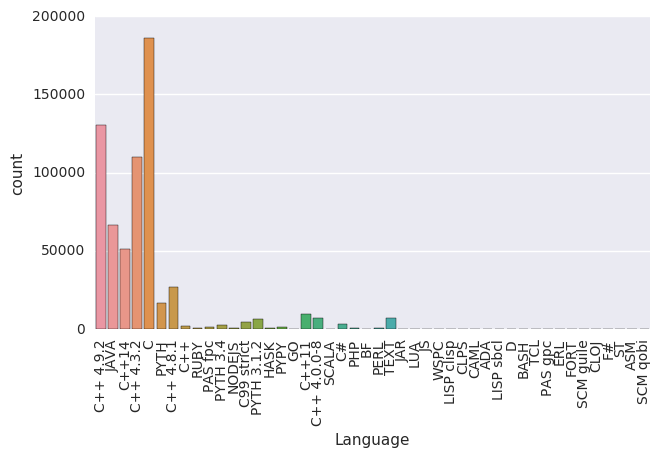
\includegraphics[width=\columnwidth]{images/languages.png}}
\caption{Frequency of each programming language that occurs in the dataset of solutions }
\label{languages}
\end{center}
\vskip -0.2in
\end{figure}

\citet{kagglekernal}

\section{Plan for Analysis and
Visualization}\label{plan-for-analysis-and-visualization}

\subsection{Description}\label{description}

Lorem ipsum dolor sit amet, consectetur adipiscing elit. Fusce porta
mauris sit amet finibus lacinia. Nunc id pharetra tortor, quis
scelerisque tellus. Nunc at est nec sapien tincidunt ultricies a quis
mi. Curabitur sed sem vitae ipsum varius molestie. Integer sed arcu
velit. Fusce ornare malesuada dolor, ut finibus arcu ornare ut. Nam
tincidunt sem in tempor pellentesque. Integer efficitur, nisl vel
euismod ultricies, nisl orci volutpat orci, nec ultrices nisi tortor id
eros.

\subsection{Technology Breakdown}\label{technology-breakdown}

Lorem ipsum dolor sit amet, consectetur adipiscing elit. Fusce porta
mauris sit amet finibus lacinia. Nunc id pharetra tortor, quis
scelerisque tellus. Nunc at est nec sapien tincidunt ultricies a quis
mi. Curabitur sed sem vitae ipsum varius molestie. Integer sed arcu
velit. Fusce ornare malesuada dolor, ut finibus arcu ornare ut. Nam
tincidunt sem in tempor pellentesque. Integer efficitur, nisl vel
euismod ultricies, nisl orci volutpat orci, nec ultrices nisi tortor id
eros.

\bibliography{bibliography.bib}
\bibliographystyle{plainnat}

\end{document} 
